\chapter{Results}
\label{chapter:results}
This chapter states the results of the proposed methods.

In section \ref{sec:model_comparison} we showed results of trained models on different stages of the dataset.

Section \ref{sec:model_improvements_results} contains results of improvements to training pipeline proposed in section \ref{sec:general_changes}.

In section \ref{sec:model_inspection_results}, we show how different backbones' sizes and weight decay affected the performance of the model.

Section \ref{sec:ensembling_results} reprots the influence of ensemble nerual networks.

Section \ref{sec:dental_restoration_results} contains results of algorithms for segmentation of dental restorations

In the final secton \ref{sec:result_comparision_with_lit} we compare results of our best-performing model with the literature.

\section{Model comparison}
\label{sec:model_comparison}
In this section we compare the performance of different model architecures and their backbones. This section is diveded into five subsection corresponging to five stages of the dataset. For each of those we report average precision metric on the test part of the dataset, unles stated otherwise.
\subsection{Stage one dataset}
\begin{table}[H]
    \centering
    \begin{tabular}{|l|c|c|c|c|c|c|}
        \hline
        Model           & $AP$  & $AP@.5$ & $AP@.75$ & $AP@.5_S$ & $AP@.5_M$ & $AP@.5_L$ \\ \hline
        FRCNN-R50       & 0.045 & 0.168   & 0.0064   & 0.109     & 0.187     & 0.141     \\ \hline
        YOLOv3          & 0.078 & 0.238   & -        & -         & -         & -         \\ \hline
        YOLOv5-l6       & 0.082 & 0.258   & 0.02     & 0.211     & 0.309     & 0.327     \\ \hline
        YOLOv5-x6       & 0.087 & 0.268   & 0.04     & 0.204     & 0.324     & 0.302     \\ \hline
        EfficientDet-d4 & 0.081 & 0.242   & 0.007    & 0.198     & 0.234     & 0.287     \\ \hline
    \end{tabular}
    \caption{Comparision of trained model on the stage one dataset}
    \label{tab:model_results:stage_one}
\end{table}

\subsection{Stage two dataset}

\begin{table}[H]
    \centering
    \begin{tabular}{|l|c|c|c|c|c|c|}
        \hline
        Model            & $AP$  & $AP@.5$ & $AP@.75$ & $AP@.5_S$ & $AP@.5_M$ & $AP@.5_L$ \\ \hline
        YOLOv3           & 0.093 & 0.258   & -        & -         & -         & -         \\ \hline
        YOLOv5 L         & 0.097 & 0.318   & 0.03     & 0.281     & 0.310     & 0.378     \\ \hline
        YOLOv5 XL        & 0.105 & 0.337   & 0.05     & 0.278     & 0.323     & 0.392     \\ \hline
        EffDet d4        & 0.089 & 0.296   & 0.01     & 0.272     & 0.291     & 0.342     \\ \hline
        EffDet d4, train & 0.421 & 0.839   & 0.362    & 0.758     & 0.852     & 0.801     \\ \hline
    \end{tabular}
    \caption{Comparision of trained model on the stage two dataset}
    \label{tab:model_results:stage_two}
\end{table}

\subsection{Stage three dataset}
Results of trained models evaluated on the training part and the test part of the dataset are available in tables \ref{tab:model_results:stage_three:train} and \ref{tab:model_results:stage_three:test}.

\begin{table}[H]
    \centering
    \begin{tabular}{|l|c|c|c|c|c|c|c|}
        \hline
        Model     & $AP$  & $AP@.3$ & $AP@.5$ & $AP@.75$ & $AP@.5_S$ & $AP@.5_M$ & $AP@.5_L$ \\ \hline
        YOLOv5-l6 & 0.463 & 0.869   & 0.841   & 0.442    & 0.697     & 0.887     & 0.974     \\ \hline
        EffDet-D4 & 0.297 & 0.82    & 0.735   & 0.164    & 0.552     & 0.838     & 0.815     \\ \hline
    \end{tabular}
    \caption{Comparision of trained models on the train part of stage three dataset}
    \label{tab:model_results:stage_three:train}
\end{table}

\begin{table}[H]
    \centering
    \begin{tabular}{|l|c|c|c|c|c|c|c|}
        \hline
        Model  & $AP$  & $AP@.3$ & $AP@.5$ & $AP@.75$ & $AP@.5_S$ & $AP@.5_M$ & $AP@.5_L$ \\ \hline
        YOLOv5 & 0.249 & 0.734   & 0.631   & 0.132    & 0.598     & 0.671     & 0.607     \\ \hline
        EffDet & 0.168 & 0.666   & 0.525   & 0.041    & 0.435     & 0.606     & 0.527     \\ \hline
    \end{tabular}
    \caption{Comparision of trained models on the test part of stage three dataset}
    \label{tab:model_results:stage_three:test}
\end{table}

% \begin{table}[H]
%     \begin{tabular}{|c|c|c|c|c|c|}
%         \hline
%         Backbone & $AP@.5$ & $AP$  & Parameters[M] & Flops[G] & Time[h] \\ \hline
%         5s6      & 0.593   & 0.231 & 12            & 21       & 2.1     \\ \hline
%         5m6      & 0.621   & 0.242 & 35            & 63       & 3.5     \\ \hline
%         5l6      & 0.611   & 0.241 & 76            & 141      & 5.2     \\ \hline
%         5x6      & 0.601   & 0.238 & 140           & 267      & 8.5     \\ \hline
%     \end{tabular}
%     \caption{Results of the YOLOv5 architecture with different backbones}
%     \label{tab:stage_three:yolov5_backbones}
% \end{table}

\subsection{Stage four dataset}
The average precision of models trained on this stage of the dataset is in table \ref{tab:model_results:stage_four}. Furthermore precision-recall values for confidence threshold maximizing F1 score are in table \ref{tab:model_prf:stage_four}, which is located in appendix.

\begin{table}[H]
    \begin{tabular}{|c|c|c|c|c|c|c|}
        \hline
        Model      & $AP$  & $AP@.5$ & $AP@.75$ & $AP@.5_S$ & $AP@.5_M$ & $AP@.5_L$ \\ \hline
        FRCNN-R101 & 0.285 & 0.675   & 0.198    & 0.568     & 0.717     & 0.772     \\ \hline
        FRCNN-R50  & 0.284 & 0.658   & 0.204    & 0.557     & 0.695     & 0.77      \\ \hline
        YOLOv5-m6  & 0.288 & 0.644   & 0.209    & 0.593     & 0.667     & 0.766     \\ \hline
        YOLOv5-l6  & 0.284 & 0.644   & 0.203    & 0.551     & 0.701     & 0.612     \\ \hline
        EffDet-D4  & 0.251 & 0.605   & 0.15     & 0.49      & 0.677     & 0.545     \\ \hline
        RetN-swint & 0.266 & 0.66    & 0.175    & 0.497     & 0.721     & 0.786     \\ \hline
        RetN-R50   & 0.263 & 0.643   & 0.174    & 0.547     & 0.696     & 0.663     \\ \hline
    \end{tabular}
    \caption{performance comparison of multiple models based on mean average precision metrics}
    \label{tab:model_results:stage_four}
\end{table}

\subsection{Stage five}

\begin{table}[H]
    \begin{tabular}{|c|c|c|c|c|c|c|c|}
        \hline
        Model      & $AP$  & $AP@.5$ & $AP@.75$ & $AP@.5_S$ & $AP@.5_M$ & $AP@.5_L$ \\ \hline
        FRCNN-R101 & 0.328 & 0.71    & 0.263    & 0.613     & 0.742     & 0.816     \\ \hline
        FRCNN-R50  & 0.334 & 0.715   & 0.273    & 0.595     & 0.757     & 0.809     \\ \hline
        YOLOv5-m6  & 0.346 & 0.708   & 0.284    & 0.622     & 0.744     & 0.754     \\ \hline
        YOLOv5-l6  & 0.295 & 0.625   & 0.232    & 0.533     & 0.691     & 0.489     \\ \hline
        EffDet-D4  & 0.288 & 0.648   & 0.219    & 0.548     & 0.699     & 0.655     \\ \hline
        RetN-swint & 0.328 & 0.72    & 0.241    & 0.565     & 0.776     & 0.775     \\ \hline
    \end{tabular}
    \caption{Performance comparison of multiple models based on mean average precision metrics}
    \label{tab:model_results:stage_five}
\end{table}

\section{Model improvements}
\label{sec:model_improvements_results}
\subsection{General improvements}
Average precision of models trained with incorporated imrpovements can be seen in table \ref{tab:improved:precision}, furthermore average recall values can be seen in table \ref{tab:improved:recall}, which is located in appednix together with table of precsion-recall values for given confidence threshold \ref{tab:imrpoved:prf}.
\begin{table}[H]
    \centering
    \begin{tabular}{|c|c|c|c|c|c|c|c|}
        \hline
        Model      & $AP$  & $AP@.3$ & $AP@.5$ & $AP@.75$ & $AP@.5_S$ & $AP@.5_M$ & $AP@.5_L$ \\ \hline
        YOLOv5-l6  & 0.347 & 0.796   & 0.725   & 0.291    & 0.597     & 0.772     & 0.753     \\ \hline
        YOLOv5-m6  & 0.343 & 0.795   & 0.719   & 0.287    & 0.636     & 0.752     & 0.785     \\ \hline
        YOLOv5-s6  & 0.327 & 0.79    & 0.697   & 0.281    & 0.559     & 0.739     & 0.826     \\ \hline
        Effdet-D1  & 0.319 & 0.787   & 0.701   & 0.251    & 0.584     & 0.752     & 0.808     \\ \hline
        FRCNN-R50  & 0.311 & 0.788   & 0.705   & 0.231    & 0.629     & 0.737     & 0.788     \\ \hline
        FRCNN-R101 & 0.316 & 0.792   & 0.688   & 0.239    & 0.563     & 0.732     & 0.793     \\ \hline
        RetN-swint & 0.325 & 0.803   & 0.723   & 0.249    & 0.579     & 0.78      & 0.758     \\ \hline
    \end{tabular}
    \caption{Comparision of AP values between different models}
    \label{tab:improved:precision}
\end{table}



\subsection{Group normalization}
Chart of $AP@.5$ for EfficientDet-D5 models with batach-normalization layers and group normlization layer is in figure \ref{fig:batch_group_diff}. Model using batch normalization achieved $AP@.5$ of 0.634 on the test dataset, beeing outperformed by model using group normalization, with $AP@.5$.
\begin{figure}[H]
    \centering
    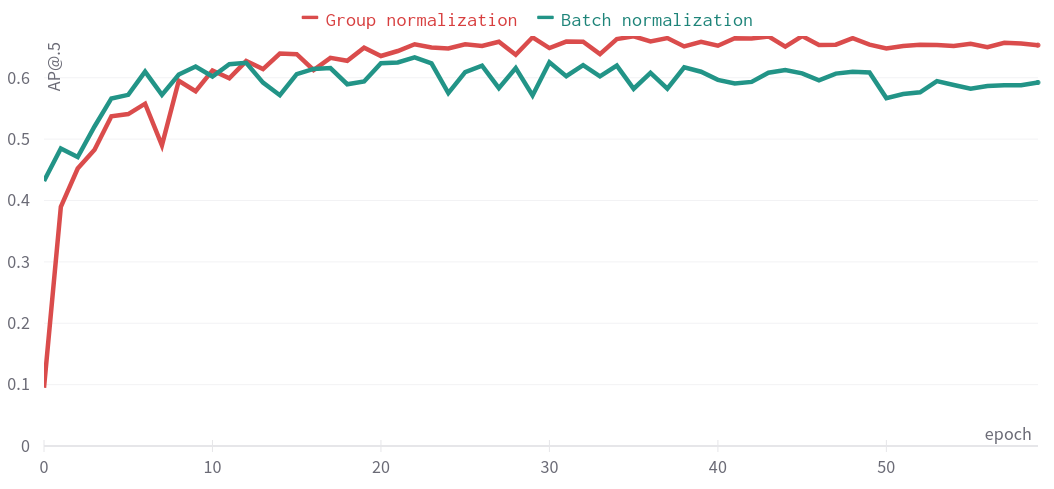
\includegraphics[width=0.9\textwidth]{images/group_norm_batch_norm.png}
    \caption{Difference in $AP@.5$ amoqEfficientDet-D5 model with batch normalization and group normalization}
    \label{fig:batch_group_diff}
\end{figure}

\section{Model inspection}
\label{sec:model_inspection_results}
\subsection{Size of backbone}
The table \ref{tab:backbone_comparison} was computed by statistics from 29 models, where each type of backbone was represented by 8 to 12 models. The columns mean, std, max and min denote statistics of $AP@.5$ obtained by trained models. Furthermore, we can inspect the size of a given backbone, which is induced by its number of parameters (Par) and floating-point operations FLOPs. The last column of table $\ref{tab:backbone_comparison}$ shows the average time required to train the given backbone.
\begin{table}[H]
    \begin{tabular}{|c|c|c|c|c|c|c|c|}
        \hline
        Backbone & Mean  & Std    & Max   & Min   & Par[M] & FLOPs[G] & Time[h] \\ \hline
        Small    & 0.68  & 0.0197 & 0.651 & 0.697 & 12     & 21       & 2.1     \\ \hline
        Medium   & 0.696 & 0.0126 & 0.669 & 0.719 & 35     & 63       & 3.5     \\ \hline
        Large    & 0.703 & 0.0136 & 0.681 & 0.725 & 76     & 141      & 5.2     \\ \hline
    \end{tabular}
    \caption{Comparision of $AP.@5$ metric for different backbones of YOLOv5 architecture}
    \label{tab:backbone_comparison}
\end{table}

\subsection{Weight decay}
In the figures \ref{fig:fasterrcnn_weight_decay} and \ref{fig:yolo_weight_decay} we see, the comparison of Faster-RCNN and YOLOv5 models using different weight decay. The results, obtained by evaluating trained models on test part of the dataset, did not differ across the values of weight decay.
\begin{figure}[H]
    \begin{floatrow}[2]
        \ffigbox[\FBwidth]{
            \caption{$AP@.5$ of Faster-RCNN model with varying weight decay values. The metric is computed on validation part of the dataset during the course of triaing.  \label{fig:fasterrcnn_weight_decay}}
        }{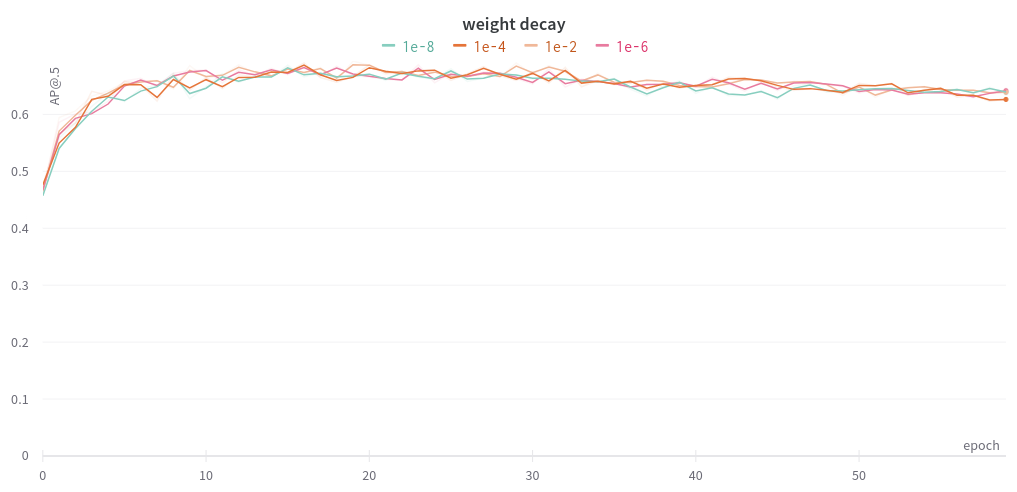
\includegraphics[width=\linewidth]{images/weight_decay_fasterrcnn.png}}
        \ffigbox[\FBwidth]{\caption{$AP@.5$ of YOLOv5 model with varying weight decay values. The metric is computed on validation part of the dataset during the course of triaing. \label{fig:yolo_weight_decay}}}
        { 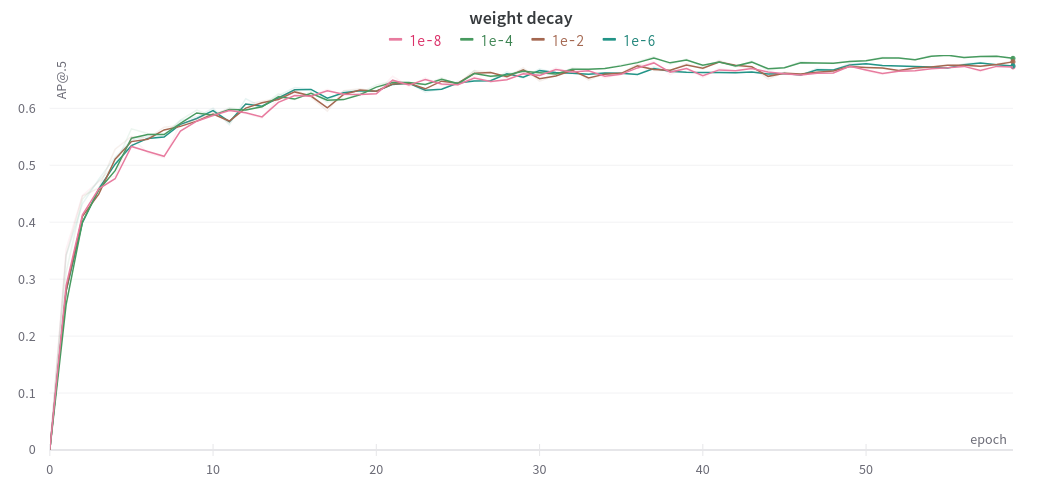
\includegraphics[width=\linewidth]{images/weight_decay_yolo.png} }
    \end{floatrow}
\end{figure}

\section{Ensembling}
\label{sec:ensembling_results}
In this section, we show the performance of model ensembles with handpicked parameters \ref{subsec:handpicked} as well as ensembles obtained by parameters found by a grid-search. Furthermore, we report how the diversity of models involved in the ensemble affects its results.
\subsection{Manually-picked parameters}
\label{subsec:handpicked}
In the table \ref{tab:model_ensembling:handpicked}, the reader can see results obtained by handpicking circa ten sets of hyper-parameters, based on our qualified quess. Than evaluating those on validation part of the dataset and selecting the best-performing, which was evaluated on test part of the dataset. The first group contained the following models trained on stage four dataset: RetinaNet-swint, YOLOv5-m, RetinaNet-ResNet50. The second group was composed of: Faster R-CNN-Resnet101, YOLOv5-m, RetinaNet-swint.
\begin{table}[H]
    \begin{tabular}{|c|c|c|c|c|c|c|c|}
        \hline
        Models & $AP$  & $AP@.3$ & $AP@.5$ & $AP@.75$ & $AP@.5_S$ & $AP@.5_M$ & $AP@.5_L$ \\ \hline
        G1     & 0.303 & 0.776   & 0.694   & 0.216    & 0.605     & 0.729     & 0.803     \\ \hline
        G2     & 0.305 & 0.783   & 0.695   & 0.218    & 0.598     & 0.733     & 0.807     \\ \hline
    \end{tabular}
    \caption{WBF ensemble of multiple models, wehre we handpicked the parameters of the ensemble process. The models were trained on stage four dataset.}
    \label{tab:model_ensembling:handpicked}
\end{table}
\subsection{Grid search results}
\label{subsec:gridsearched}
The best hyper-parameters for a given ensemble method found by a grid search are in the table \ref{tab:ensemble_params:grid_search}. We omitted from the table parameter $\sigma$, used only in S-NMS. Its optimal value, according to the grid search, was $0.8$.
Average precision of the models ensembled with parameters from table \ref{tab:ensemble_params:grid_search} is available in the table \ref{tab:precision:grid_search} and average recall values are in the table \ref{tab:recall:grid_search}. Precison and recall values based on the confidence threshold, that maximizes F-score can be seen in table \ref{tab:ensembling_prf:grid_search}.

\begin{table}[H]
    \begin{tabular}{|c|c|c|c|c|c|c|}
        \hline
        Method  & FRCNN & YOLOv5 & RetN  & FRCNN & $T$  \\
                & R50   & m6     & swint & R101  &      \\ \hline
        NMS     & 1     & 0.4    & 0.4   & 0.85  & 0.6  \\ \hline
        SNMS    & 1     & 0.12   & 0.12  & 0.12  & 0.7  \\ \hline
        NMW     & 0.85  & 0.25   & 0.70  & 0.85  & 0.45 \\ \hline
        WBF     & 1     & 0.4    & 0.85  & 0.85  & 0.65 \\ \hline
        WBF-A S & 0.94  & 0.31   & 0.98  & 0.72  & 0.64 \\ \hline
        WBF-A M & 0.77  & 0.47   & 0.85  & 0.69  & 0.64 \\ \hline
        WBF-A L & 0.84  & 0.31   & 0.88  & 0.91  & 0.64 \\ \hline
    \end{tabular}
    \caption{Hyper-parameter values of ensemble methods found by a grid-seach}
    \label{tab:ensemble_params:grid_search}
\end{table}


\begin{table}[H]
    \centering
    \begin{tabular}{|c|c|c|c|c|c|c|c|}
        \hline
        Method & $AP$  & $AP@.3$ & $AP@.5$ & $AP@.75$ & $AP@.5_S$ & $AP@.5_M$ & $AP@.5_L$ \\ \hline
        NMS    & 0.346 & 0.818   & 0.735   & 0.28     & 0.618     & 0.775     & 0.829     \\ \hline
        SNMS   & 0.348 & 0.807   & 0.722   & 0.295    & 0.609     & 0.758     & 0.819     \\ \hline
        NWM    & 0.364 & 0.829   & 0.759   & 0.302    & 0.641     & 0.802     & 0.854     \\ \hline
        WBF    & 0.378 & 0.832   & 0.77    & 0.323    & 0.663     & 0.807     & 0.875     \\ \hline
        WBF-A  & 0.376 & 0.832   & 0.768   & 0.318    & 0.651     & 0.806     & 0.875     \\ \hline
    \end{tabular}
    \caption{Average precision of models ensembled by parameters from table \ref{tab:ensemble_params:grid_search}}
    \label{tab:precision:grid_search}
\end{table}


\subsection{Assesing importance of different models}
In tables \ref{tab:precision:ensemble_compare}, \ref{tab:recall:ensemble_compare} and \ref{tab:ensembling_prf:ensemble compare} we se results of ensebmles composed of different models. Note, that ensembling of varying architectures achieved the best results out of all models evaluated in this thesis. The importance of individual models in the ensemble is in figure \ref{fig:ensembling_parameters_importance} for all architectures and in figures \ref{fig:ensembling_hparams_imprtance_yolo_m}, \ref{fig:ensembling_hparams_imprtance_yolo_mix} located in appendix for the remaining two groups of models.

\begin{table}[h]
    \centering
    \begin{tabular}{|c|c|c|c|c|c|c|c|}
        \hline
        Models & $AP$  & $AP@.3$ & $AP@.5$ & $AP@.75$ & $AP@.5_S$ & $AP@.5_M$ & $AP@.5_L$ \\ \hline
        All    & 0.389 & 0.838   & 0.774   & 0.338    & 0.665     & 0.811     & 0.876     \\ \hline
        Y5-mix & 0.379 & 0.819   & 0.75    & 0.34     & 0.636     & 0.79      & 0.84      \\ \hline
        Y5-m   & 0.368 & 0.812   & 0.741   & 0.329    & 0.648     & 0.775     & 0.844     \\ \hline
    \end{tabular}
    \caption{Average precision of ensembled models}
    \label{tab:precision:ensemble_compare}
\end{table}


\begin{table}[h]
    \centering
    \begin{tabular}{|c|c|c|c|c|c|c|c|}
        \hline
        Models & $AR$  & $AR@.5_{10}$ & $AR@.5$ & $AR@.75$ & $AR@.5_S$ & $AR@.5_M$ & $AR@.5_L$ \\ \hline
        All    & 0.586 & 0.917        & 0.978   & 0.582    & 0.946     & 0.991     & 0.991     \\ \hline
        Y5-mix & 0.579 & 0.911        & 0.959   & 0.599    & 0.929     & 0.972     & 0.972     \\ \hline
        Y5-m   & 0.562 & 0.906        & 0.949   & 0.572    & 0.909     & 0.964     & 0.964     \\ \hline
    \end{tabular}
    \caption{Average recall of models ensembled by parameters from table \ref{tab:ensemble_params:grid_search}}
    \label{tab:recall:ensemble_compare}
\end{table}


\begin{table}[h]
    \begin{tabular}{|c|c|c|c|c|}
        \hline
        Models     & Precision & Recall & F-score & Confidence threshold \\ \hline
        All        & 0.751     & 0.7    & 0.725   & 0.294                \\ \hline
        YOLOv5-mix & 0.728     & 0.69   & 0.708   & 0.241                \\ \hline
        YOLOv5-m   & 0.726     & 0.67   & 0.697   & 0.272                \\ \hline
    \end{tabular}
    \caption{Precision, recall, and F-score based on the confidence threshold for different ensembling methods}
    \label{tab:ensembling_prf:ensemble compare}
\end{table}

\begin{figure}
    \centering
    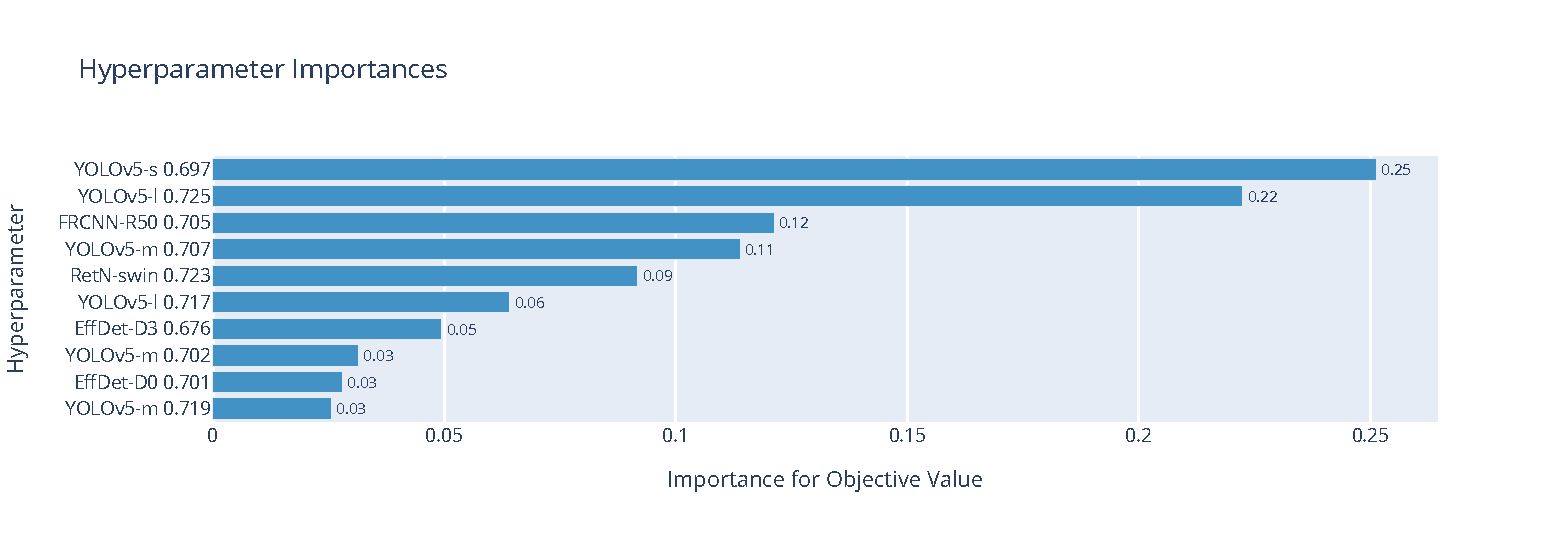
\includegraphics[width=\linewidth]{images/ensemble_all_importance.pdf}
    \caption{Importance of different models during ensembling with different architectures}
    \label{fig:ensembling_parameters_importance}
\end{figure}


\begin{figure}[H]
    \begin{floatrow}[2]
        \ffigbox[\FBwidth]{
            \caption{Number of false positives per image for given value of recall \label{fig:recall_fiperimg}}
        }{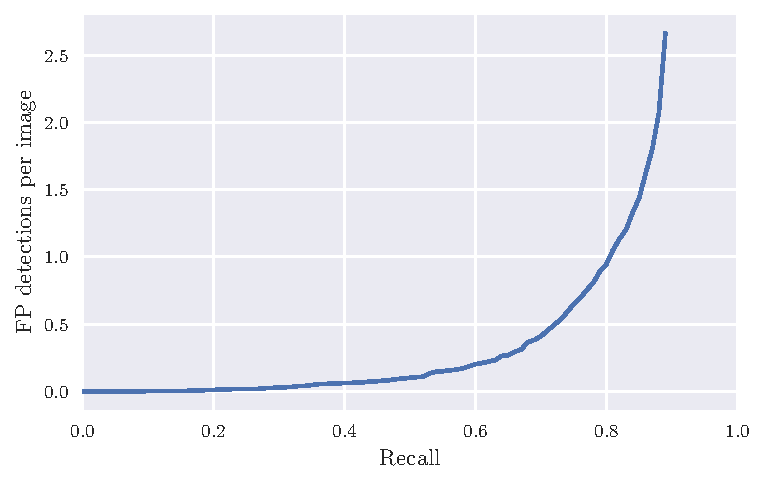
\includegraphics[width=\linewidth]{images/fp_recall.pdf}}
        \ffigbox[\FBwidth]{\caption{Percentage of nondetected dental caries based on the precision of the model}}
        { 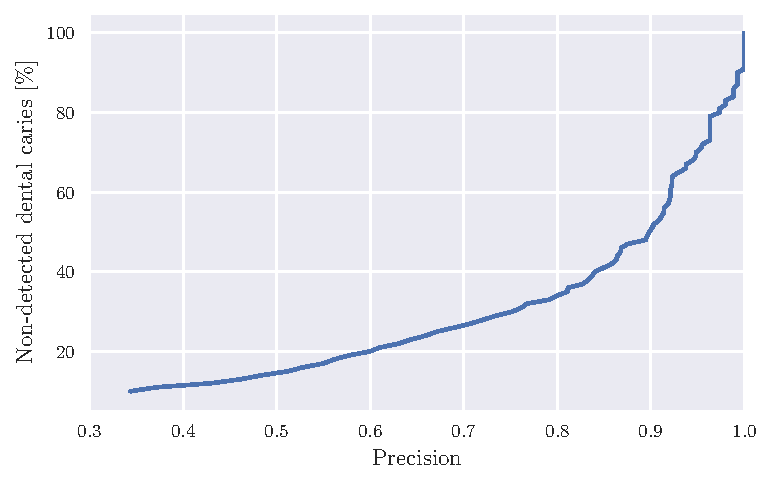
\includegraphics[width=\linewidth]{images/nondet_precision.pdf} }
    \end{floatrow}
\end{figure}

\section{Dental retorations segmentation}
\label{sec:dental_restoration_results}
\subsection{Non-deeplearning approach}
Hyper-parameters ensuring the best performance on validation part of the datset are in table \ref{tab:nondl_restorations:best_params}. Performance of the pipelie on test dataset given the parameters in the table \ref{tab:nondl_restorations:best_params} can be seen in table \ref{tab:nondl_results}. Segmentation of an image together with output after each auxilary stage is in figure \ref{fig:segmentation_sample_nondl}.

\begin{figure}[h]
    \centering
    \begin{subfigure}[b]{\textwidth}
        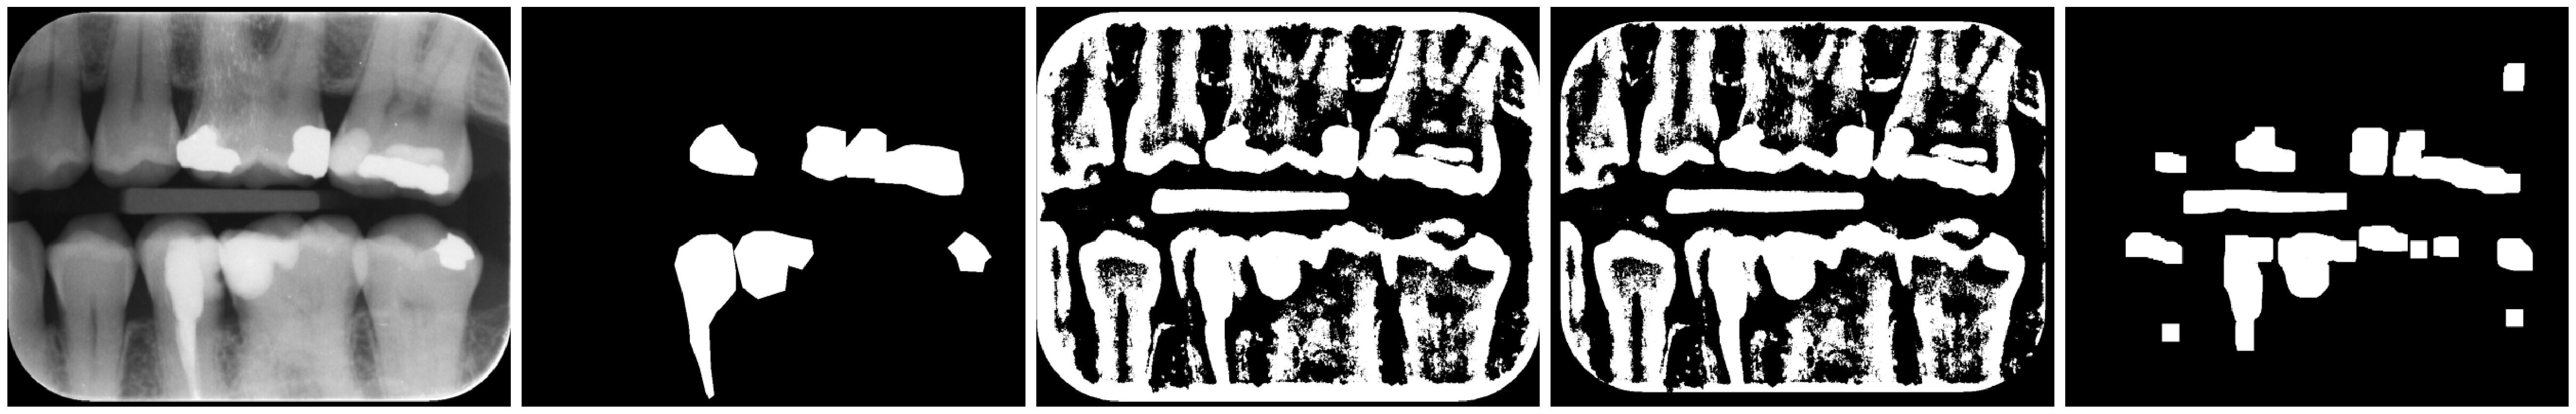
\includegraphics[width=1\linewidth]{images/segmentation_nondl_gauss_12.pdf}
        \caption{Gaussian adaptive thresholding}
    \end{subfigure}

    \begin{subfigure}[b]{\textwidth}
        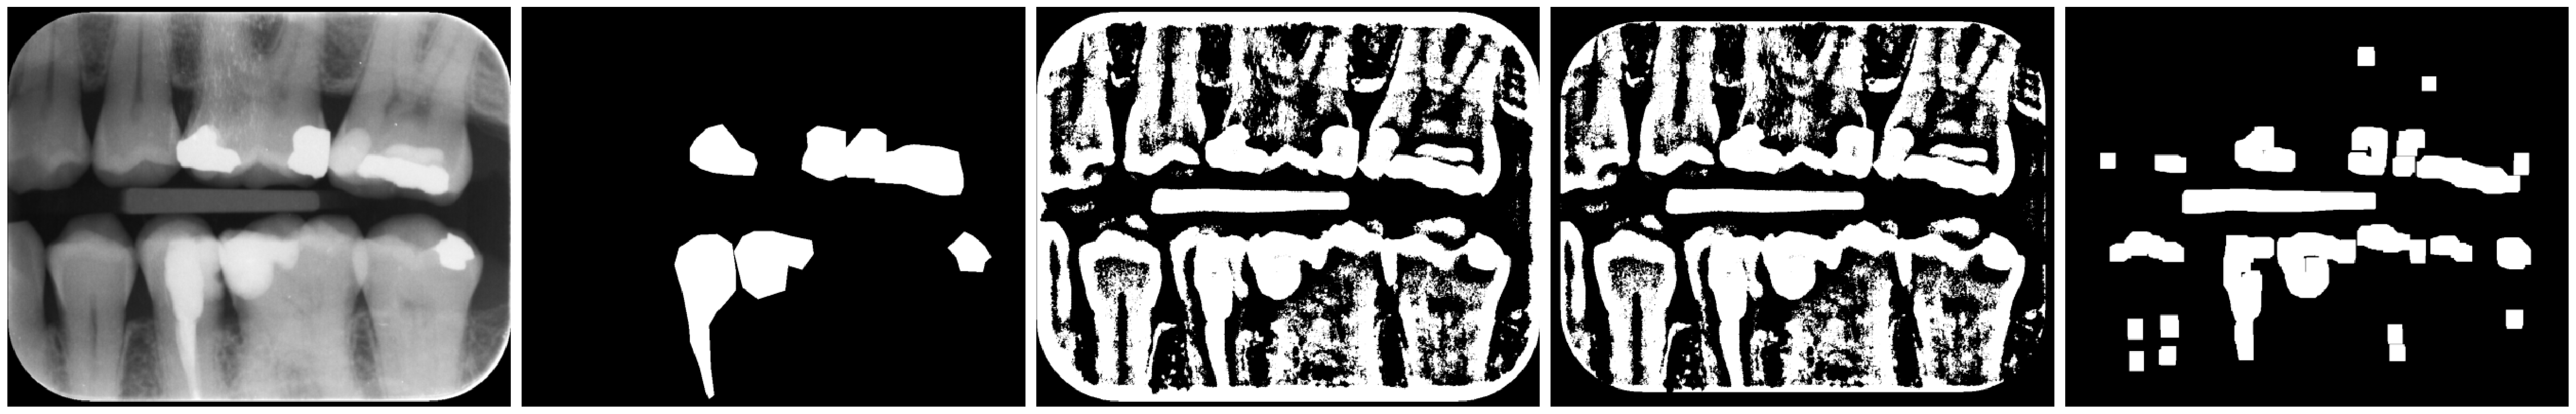
\includegraphics[width=1\linewidth]{images/segmentation_nondl_mean_12.pdf}
        \caption{Mean adaptive thresholding}
    \end{subfigure}
    \caption{From the left: X-ray image, ground-truth pixel mask, thresholded image, removal of border pixels, morphological opening}
    \label{fig:segmentation_sample_nondl}
\end{figure}

\begin{table}[H]
    \begin{tabular}{|c|c|c|c|}
        \hline
        Hyper-parameter & Adaptive mean & Adaptive Gaussian & Otsu's \\ \hline
        $K_t$           & 71            & 83                & -      \\ \hline
        $T$             & 3             & 3                 & -      \\ \hline
        $K_d$           & 41            & 41                & 61     \\ \hline
        $K_o$           & 31            & 36                & 36     \\ \hline
        $K_b$           & -             & -                 & 21     \\ \hline
    \end{tabular}
    \caption{Best hyper-parameters for non-deeplerning pipeline}
    \label{tab:nondl_restorations:best_params}
\end{table}


\begin{table}[H]
    \centering
    \begin{tabular}{|c|c|c|}
        \hline
        Model               & Dice  & IOU   \\ \hline
        Adaptive mean       & 0.364 & 0.314 \\ \hline
        Adaptive Gaussian   & 0.328 & 0.274 \\ \hline
        Otus's thresholding & 0.102 & 0.088 \\ \hline
    \end{tabular}
    \caption{Results of non-deeplerning approach to dental resotrations segmentation given the hyper-parameters in table \ref{tab:nondl_restorations:best_params}}
    \label{tab:nondl_results}
\end{table}



\subsection{U-Net}
Two U-Net models were trained; we will call them U-Net-baseline (U-Net-B) and U-Net-improved (U-Net-I). With the letters PP, we denote that output of the model was post-processed by the approach described in section \ref{sec:segmentation_post_processing}.

The best hyper-parameters for post-processing for both models are in table \ref{tab:unet_seg_hyperparams}. In figure \ref{fig:heatmap_postprocess} is visible, how choice of different hyper-parameters for post-procssing pipeline affected the performance of U-Net-B model.

Figure \ref{fig:segmentation_unet_sample} shows results of segmentation and compares those with ground truth mask.

\begin{figure}[h]
    \centering
    \begin{subfigure}[b]{\textwidth}
        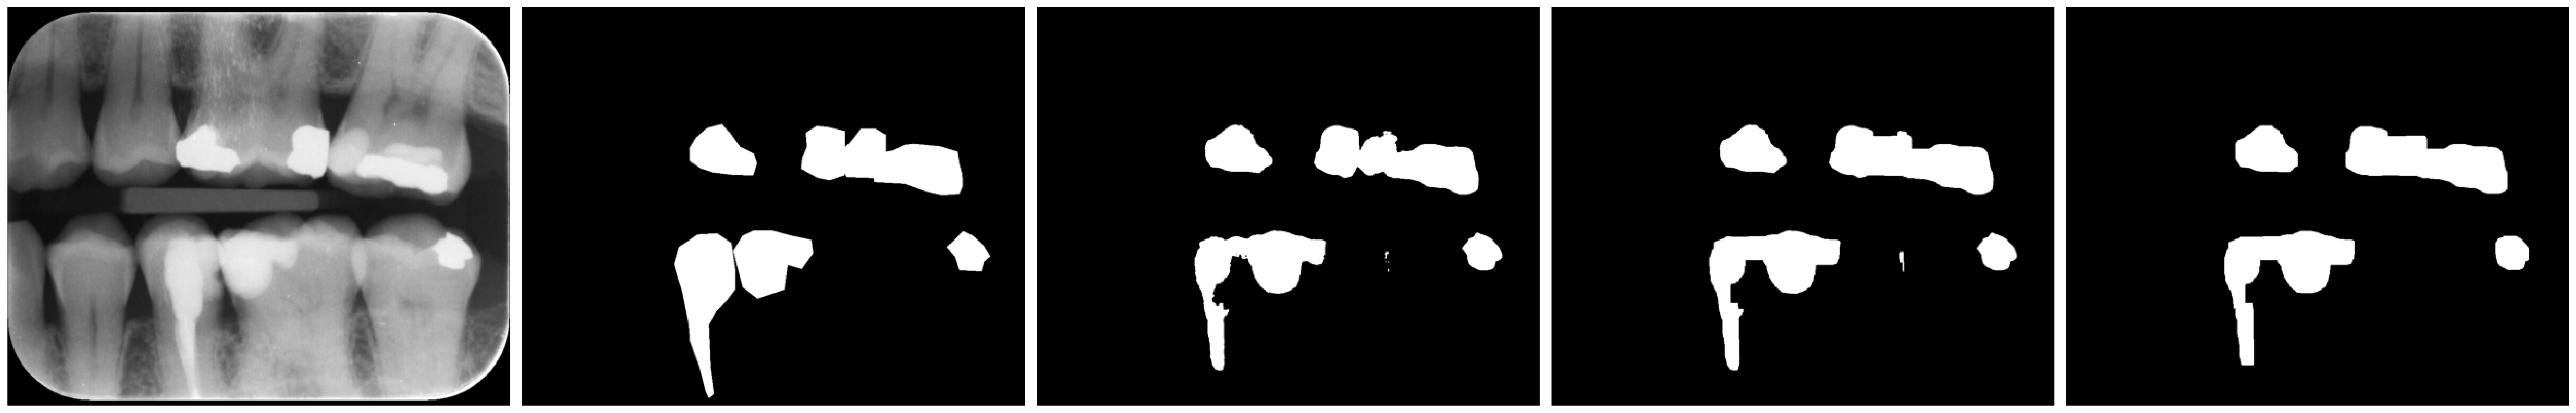
\includegraphics[width=1\linewidth]{images/unet_1_img_12.pdf}
        \caption{Baseline U-Net model}
    \end{subfigure}

    \begin{subfigure}[b]{\textwidth}
        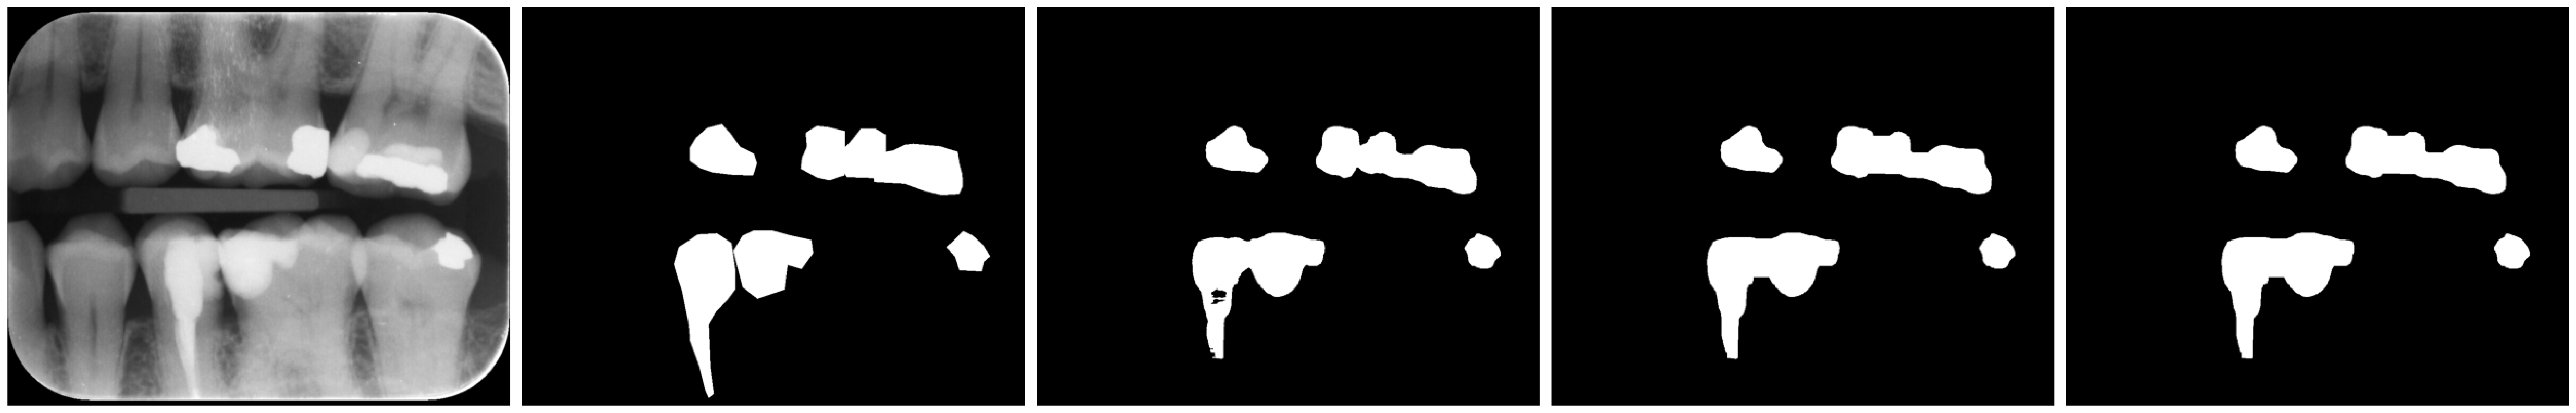
\includegraphics[width=1\linewidth]{images/unet_2_img_12.pdf}
        \caption{Imrpoved U-Net model}
    \end{subfigure}
    \caption{From the left: X-ray image, ground-truth pixel mask, output of the model, output processed by morphological opening, output post-processed by morphological opening and closing.}
    \label{fig:segmentation_unet_sample}
\end{figure}
\begin{figure}
    \centering
    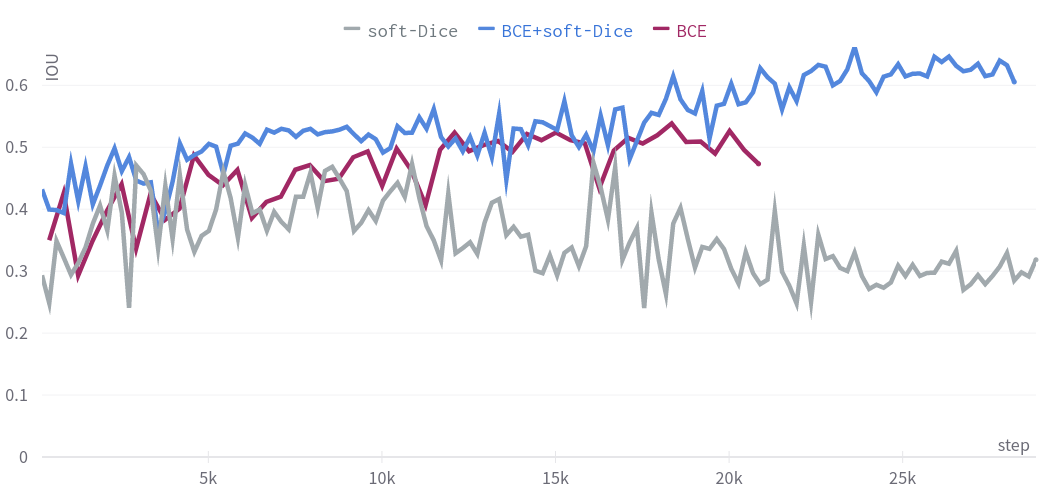
\includegraphics[width=0.8\linewidth]{images/segmentation_losses.png}
    \caption{IOU throughout the training of U-Net model for different losse functions}
    \label{fig:segmentation_losses}
\end{figure}

\begin{figure}[H]
    \centering
    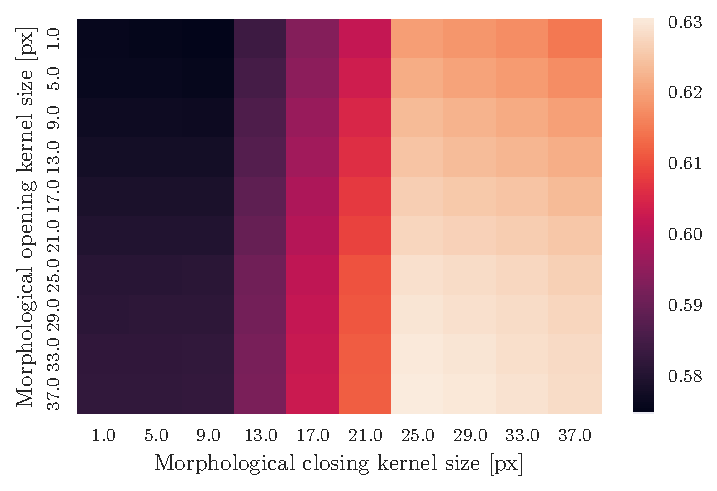
\includegraphics[]{images/heatmap_of_unetpostproc_search.pdf}
    \caption{Value of IOU metric based on the size of kernels $K_o$, $K_c$ in morphological operations, that were used for post-processing}
    \label{fig:heatmap_postprocess}
\end{figure}

\begin{minipage}{\textwidth}

    \begin{minipage}[t]{0.48\textwidth}
        \centering
        \makeatletter\def\@captype{table}
        \begin{tabular}{|c|c|c|}
            \hline
            Parameter & $K_o$ & $K_c$ \\ \hline
            U-Net     & 37    & 25    \\ \hline
            U-Net-I   & 33    & 5     \\ \hline
        \end{tabular}
        \caption{Optimal parameters for model post-processing found by a grid-search}
        \label{tab:unet_seg_hyperparams}
    \end{minipage}
    \begin{minipage}[t]{0.48\textwidth}
        \centering
        \makeatletter\def\@captype{table}
        \begin{tabular}{|c|c|c|}
            \hline
            Model      & Dice  & IOU   \\ \hline
            U-Net-B    & 0.663 & 0.575 \\ \hline
            U-Net-B-PP & 0.714 & 0.623 \\ \hline
            U-Net-I    & 0.747 & 0.662 \\ \hline
            U-Net-I-PP & 0.760 & 0.676 \\ \hline
        \end{tabular}
        \caption{Results of U-Net models}
        \label{tab:unet_seg_results}
    \end{minipage}
\end{minipage}


\section{Comparision of results with related publications}
\label{sec:result_comparision_with_lit}
% \subsection{Caries detection}
In the table \ref{tab:results_comparison}, we see a comparison of the results of this thesis with results achieved by related works. We compared with only those who selected a similar approach to ensure at least a minimal amount of comparability.

\begin{table}
    \centering
    \begin{tabular}{|c|c|c|c|c|c|}
        \hline
        Author                                                                 & Precision & Recall & F1-Score & Accuracy & $AP@.5$ \\ \hline
        This thesis                                                            & 0.751     & 0.7    & 0.725    & 0.726    & 0.774   \\ \hline
        Srivastava et al. \cite{Srivastava2017}                                & 0.615     & 0.805  & 0.7      & -        & -       \\ \hline
        Kumar                                   \& Srivastava \cite{Kumar2018} & 0.7       & 0.53   & 0.614    & -        & -       \\ \hline
        Bayrakdar et al. \cite{Bayrakdar2021}                                  & 0.78      & 0.77   & 0.78     & -        & -       \\ \hline
        Bayraktar et al. \cite{Bayraktar2021}                                  & -         & 0.72   & -        & 0.946    & 0.872   \\ \hline
        Cantu et al. \cite{Cantu2020}                                          & -         & 0.75   & 0.73     & 0.8      & -       \\ \hline
    \end{tabular}
    \caption{Comparison of results of this thesis with results in related publications}
    \label{tab:results_comparison}
\end{table}

Note that Cantu et al. \cite{Cantu2020} solved the problem of dental caries localization as a semantic segmentation task; the recall and F1-score are calculated per pixel, while other works worked with bounding boxes. However, the reader can still estimate how their work compares to others in the table.














% \begin{table}[H]
%     \begin{tabular}{|c|c|c|c|c|c|c|c|}
%         \hline
%         Model      & $AP$  & $AP@.3$ & $AP@.5$ & $AP@.75$ & $AP@.5_S$ & $AP@.5_M$ & $AP@.5_L$ \\ \hline
%         FRCNN-R101 & 0.285 & 0.763   & 0.675   & 0.198    & 0.568     & 0.717     & 0.772     \\ \hline
%         FRCNN-R50  & 0.284 & 0.76    & 0.658   & 0.204    & 0.557     & 0.695     & 0.77      \\ \hline
%         YOLOv5-m6  & 0.288 & 0.748   & 0.644   & 0.209    & 0.593     & 0.667     & 0.766     \\ \hline
%         YOLOv5-l6  & 0.284 & 0.74    & 0.644   & 0.203    & 0.551     & 0.701     & 0.612     \\ \hline
%         EffDet-D4  & 0.251 & 0.716   & 0.605   & 0.15     & 0.49      & 0.677     & 0.545     \\ \hline
%         RetN-swint & 0.266 & 0.766   & 0.66    & 0.175    & 0.497     & 0.721     & 0.786     \\ \hline
%         RetN-R50   & 0.263 & 0.734   & 0.643   & 0.174    & 0.547     & 0.696     & 0.663     \\ \hline
%     \end{tabular}
%     \caption{performance comparison of multiple models based on mean average precision metrics}
%     \label{tab:model_results:stage_four}
% \end{table}


% \begin{table}[H]
%     \begin{tabular}{|c|c|c|c|c|c|c|c|}
%         \hline
%         Model      & $AP$  & $AP@.3$ & $AP@.5$ & $AP@.75$ & $AP@.5_S$ & $AP@.5_M$ & $AP@.5_L$ \\ \hline
%         FRCNN-R101 & 0.328 & 0.8     & 0.71    & 0.263    & 0.613     & 0.742     & 0.816     \\ \hline
%         FRCNN-R50  & 0.334 & 0.81    & 0.715   & 0.273    & 0.595     & 0.757     & 0.809     \\ \hline
%         YOLOv5-m6  & 0.346 & 0.787   & 0.708   & 0.284    & 0.622     & 0.744     & 0.754     \\ \hline
%         YOLOv5-l6  & 0.295 & 0.706   & 0.625   & 0.232    & 0.533     & 0.691     & 0.489     \\ \hline
%         EffDet-d4  & 0.288 & 0.745   & 0.648   & 0.219    & 0.548     & 0.699     & 0.655     \\ \hline
%         RetN-swint & 0.328 & 0.805   & 0.72    & 0.241    & 0.565     & 0.776     & 0.775     \\ \hline
%     \end{tabular}
%     \caption{Performance comparison of multiple models based on mean average precision metrics}
%     \label{tab:model_results:stage_five}
% \end{table}